\section{Laser}\label{sec:laser}

A técnica de reconstrução baseada em laser é conhecida desde o século passado, pois oferecem uma alta qualidade geométrica de dados, os resultados são em tempo real e requer pouco tempo de captura de dados. 

Existem alguns tipos de reconstruções empregando lasers, baseados em volume (ressonância, tomografia, por exemplo \ref{fig:laservolume} ou em superfície (estereoscopia, {\it time of flight}, luz estruturada) . Neste caso, abordaremos o projeto de escaneamento da escultura de Michelangelo, David, que utiliza escaners baseados em superfícies, mais especificamente, utilizando luz estruturada.

\begin{figure}[!h]
	\centering
	%   \includegraphics[width=1.0\linewidth]{figs/3d-curve-sketch/system-diagram.eps}
	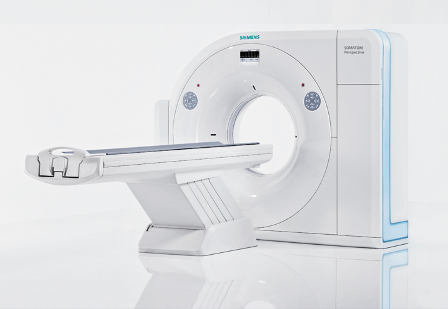
\includegraphics[width=1\linewidth]{figs/tomografia.png}
	\caption{%
	Exemplo de reconstrução à laser utilizando o método baseado em volume.
	%\cite{Cui:Theobalt:etal:PAMI2013,Pajdla:etal:ICCV2011}.
	}\label{fig:laservolume}
\end{figure}

Este projeto tem como motivação avançar a tecnologia de digitalização 3D e criar um acervo digital sobre alguns dos principais artefatos culturais. Foi utilizada uma tecnologia chamada de {\it rangefinder}, com uma equipe de mais de 30 professores, funcionários e estudantes da Universidade de Stanford desenvolveram algoritmos para combinar imagens de múltiplas gamas e cores, passaram os anos de 1998 e 1999 na Itália escaneando esclturas de Michelangelo. 

O projeto não teve mais nenhum avanço desde o verão de 2004, por falta de financiamento. Como resultado, modelos de alta qualidade só existem do David na resolução de 1,0 mm (56 milhões de triângulos) e São Mateus a 0,25 mm (372 milhões de triângulos). Um modelo também existe para o Atlas em 0,25 mm (aproximadamente 500 milhões de triângulos), mas contém erros de alinhamento. Após 6 anos de trabalho estudantil remunerado e voluntário, existem modelos para cada um dos 1.186 fragmentos. Esses modelos, que totalizam quase 8 bilhões de polígonos, se encontram no próprio site da Universidade de Stanford %CITAR AQUI$. 
Também foram disponibilizadas algumas métricas sobre este projeto \ref{tab:metricasDavid}.

\begin{table}
\caption{Algumas métricas do projeto}
\label{tab:metricasDavid}
\begin{tabular}{|l|l|}
\hline
Números de objetos escaneados             & 10 estátuas + 2 edificações + 1,163 fragmentos de mapa     \\ \hline
Menor e maior objetos escaneados       & 1 polegada (fragmentos de mapa) e 23 pés (David)       \\ \hline
Resolução espacial dos dados                & 0.29mm para geometria, 0.125mm para cor              \\ \hline
Complexidade do maior conjunto de dados             & 2 bilhões de polígonos + 7,000 imagens (David)       \\ \hline
Tamanho do maior conjunto de dados                    & 32 {\it gigabytes} (David)                            \\ \hline
Quantia total de dados capturados              & 250 {\it gigabytes}                                       \\ \hline
Tamanho do maior escaner                    & 24 pés de altura, 1800 libras de peso                           \\ \hline
Peso total do equipamento levado para a Itália & 4 toneladas                                              \\ \hline
Número de pessoas envolvidas                  & 32 (sem incluir subcontratantes e colaboradores) \\ \hline
Tempo médio para escaneamento              & 1 semana (exceto o David, que levou 1 mês)       \\ \hline
Tempo total de escaneamento                 & 5,000 horas de trabalho                                   \\ \hline
Total de tempo para processamento de dados          & 4,000 horas de trabalho (até agora)                            \\ \hline
Custo do projeto                          & \$2,000,000                                         \\ \hline
\end{tabular}

\end{table}

Porém, devido ao seu alto custo com equipamentos, com {\it softwares} e sem falar na necessidade de estações robustas para armazenamento dos dados e para esacaneamento de parimônios, outras técnicas foram emergindo com o passar dos anos, como a fotogrametria, que será abordada posteriormente.